\documentclass[12pt,a4paper]{article}
\usepackage[T1]{fontenc}
\usepackage[utf8]{inputenc}
\usepackage{lmodern}
\usepackage[a4paper,margin=2.55cm]{geometry}
\usepackage{amsmath,amssymb}
\usepackage{graphicx}
\usepackage{booktabs}
\usepackage[font=small,labelfont=bf]{caption}
\usepackage{xurl}
\usepackage[hidelinks]{hyperref}
\graphicspath{{images/}}

\newcommand{\pinv}{\operatorname{pinv}}
\newcommand{\ms}{m_n^-}
\newcommand{\vs}{v_n^-}

% ---- Title-page data (edit here) -------------------------------------
\newcommand{\reporttitle}{FR3 Simulation: Baseline and Full-Online\\ HQP Controllers}
\newcommand{\reportdegree}{Master's Degree in Control Engineering}
\newcommand{\academicyear}{2025/2026}
% ----------------------------------------------------------------------

\begin{document}

% Sapienza Universita di Roma -- title page (DIAG)
% Edit title, degree, date and academic year in main.tex.
\begin{titlepage}
  \centering
  \vspace*{-0.6cm}
  
\includegraphics[width=0.48\textwidth]{sapienza_logo}\par
  \vspace{1.9cm}
  {\large\scshape Department of Computer, Control and Management\\ Engineering\par}
  \vspace{3.4cm}
  {\LARGE\bfseries \reporttitle\par}
  \vspace{0.9cm}
  {\Large\scshape \reportdegree\par}
  \vspace{0.6cm}
  {\normalsize \reportdate\par}
  \vspace{2.4cm}
  \begin{minipage}[t]{0.42\textwidth}
    \raggedright
    {\large\bfseries Professor:\par}\vspace{0.35cm}
    Alessandro De Luca\par\vspace{0.6cm}
    {\large\bfseries Co-supervisor:\par}\vspace{0.35cm}
    Mattia Castelmare
  \end{minipage}%
  \begin{minipage}[t]{0.38\textwidth}
    \raggedright
    {\large\bfseries Students:\par}\vspace{0.35cm}
    Lorenzo Carlino\\
    Samuele Leonardi\\
    Gurwinder Sharma
  \end{minipage}
  \vfill
  \rule{\textwidth}{0.6pt}\par
  \vspace{0.6cm}
  Academic Year \academicyear\par
  \vspace{2.3cm}
\end{titlepage}

\setcounter{page}{1}
\tableofcontents
\newpage

% =====================================================================
\section{Introduction}
The main goal of this project is to investigate whether the FR3 manipulator can use its kinematic redundancy to
reduce its directional effective mass before impact. Effective mass optimization
is a secondary task in a torque controller based on hierarchical quadratic
programming (HQP). We compare it with a baseline Cartesian tracking controller
on circular and perpendicular trajectories.
The target is a reduction of at least 30\% in directional effective mass at first contact.

At first impact, the full-online controller reduced the directional effective mass by
\textbf{35.69\%} for the circular trajectory and \textbf{32.02\%} for the
perpendicular trajectory. The pre-impact normal velocities are nearly equal within
each pair, limiting the influence of impact speed on the comparison. The measured
loads also reflect differences in redundancy resolution, damping and constraints,
so these trials cannot isolate the contribution of mass optimization.

% =====================================================================
\section{Experimental Setup and Metrics}
\label{sec:setup}
Both experiments use the seven-joint FR3 model with initial configuration
\begin{equation}
  q_0 = [0,\ -0.1517,\ 0,\ -2.6105,\ 0,\ 4.0295,\ 0.785]^{\mathsf T}\ \text{rad}.
\end{equation}

The fingertip starts near $(0.56, 0, 0.50)$\,m. The wall lies in the plane
$x = 0.62$\,m, with outward normal $n = [-1, 0, 0]^{\mathsf T}$, stiffness
$20\,000$\,N/m and damping $15$\,N\,s/m. Normal velocity is positive toward the wall.
The data come from nominal simulations with measurement noise, mass errors and
joint friction disabled. The two comparisons use a 1000\,Hz controller and a
real-time factor (RTF) of 0.20. The circular pair spans 20 simulated seconds with
the same return schedule. The perpendicular pair comes from the same gain study
and uses $k_m=4$ and $k_{\mathrm{ns}}=12$ in the full-online run. Both perpendicular trials
complete the approach and endpoint hold after about 0.57\,s, within the 2\,s launch
limit. The perpendicular results use the recorded run-relative timestamps. The
first sample is at 0.007\,s in both trials.

The circular reference follows a vertical circle in the $x$--$z$ plane with a radius of
0.04\,m and a cruise period of 2\,s. With the 1\,s angular startup ramp, one
revolution from rest takes 2.5\,s. The perpendicular reference reaches
0.20\,m/s after a 0.10\,s speed ramp. It brakes over the last 4\,mm and holds the
endpoint for 0.15\,s. The desired Cartesian endpoint is set 10\,mm beyond the wall,
with actual penetration measured from the simulated motion.

The analysis uses \texttt{first\_impact} to identify the first sample with $F_n > 0$
as the start of contact. The first compression-release cycle ends at detachment or
when recompression begins in the simulation, whichever occurs first. The force,
impulse and penetration reported for that cycle cover this interval.

The pre-impact effective mass and normal velocity come from the last sample before
contact. The pre-impact normal kinetic energy and the first-cycle normal impulse are
\begin{equation}
  E_n^- = \frac{1}{2}\, \ms \left(\vs\right)^2, \qquad
  I_n = \int_{t_c}^{t_e} F_n(t)\, dt .
\end{equation}

The impulse is integrated with the trapezoidal rule at the saved timestamps.
The tables report time-weighted RMS tracking error over the pre-impact interval.
Pre-impact metrics require a preceding sample. Limit checks cover the saved samples.

% =====================================================================
\section{Controller Formulation}

\subsection{Shared Cartesian tracking law}
Let $J = \partial p/\partial q$, $e = p_d - p$ and $\dot e = v_d - J\dot q$. All four
controllers use the same Cartesian acceleration law
\begin{equation}
  a_{\mathrm{trk}} = a_d + K_p e + K_d \dot e, \qquad
  b = a_{\mathrm{trk}} - \dot J \dot q .
\end{equation}
The task specifies the three coordinates of the fingertip. When $J$ has full row
rank, the seven-joint arm has four redundant degrees of freedom for secondary
objectives. All four controllers use the same acceleration-level gains,
$K_p=100\,\mathrm{s}^{-2}$ and $K_d=20\,\mathrm{s}^{-1}$.

\subsection{Baseline controllers}
The baseline uses the Euclidean pseudoinverse and its null-space projector to compute
the joint acceleration and actuator command.
\begin{gather}
  J^\dagger = \pinv(J), \qquad N_E = I - J^\dagger J, \\
  u_B = J^\dagger b + N_E \bigl( 25 (q_0 - q) - 10\, \dot q \bigr), \qquad
  \tau_{\mathrm{cmd}} = M(q)\, u_B + c(q, \dot q).
\end{gather}
Here $c = C(q,\dot q)\dot q$. Posture feedback and damping govern the null-space
motion throughout the run. Directional effective mass is evaluated for reporting.
The simulation framework clips the commanded torque and enforces the stop conditions.
Contact force acts as an external disturbance.

\texttt{baseline\_perp.py} uses the same law with the perpendicular reference. The simulator
supplies gravity compensation $g$ separately from the actuator command.

\subsection{Full-online optimized controllers}
The optimized controllers use the dynamically consistent inverse and its
null-space projector~\cite{khatib1987}.
\begin{equation}
  \bar J = M^{-1} J^{\mathsf T} \left( J M^{-1} J^{\mathsf T} \right)^{-1}, \qquad
  N = I - \bar J J .
\end{equation}
The secondary torque preference follows the gradient of the directional effective
mass~\cite{haddadin2017}.
\begin{equation}
  m_n(q) = \frac{1}{n^{\mathsf T} J M^{-1} J^{\mathsf T} n}, \qquad
  \tau_m = -\rho(t)\, k_m\, N^{\mathsf T} \nabla_q m_n(q).
\end{equation}
The controller evaluates the gradient analytically at the current joint
configuration without normalization. Under nominal dynamics and full task rank,
the projected torque satisfies $J M^{-1} \tau_m = 0$. The HQP enforces the joint
and torque constraints.

We also tested hybrid HQP variants on both trajectories. They combined the online
effective mass gradient with a fixed posture $q^*$ computed offline with SLSQP at the
nominal contact point. The controller used this posture as an additional null-space
preference.

\begin{table}[htbp]
  \centering
  \small
  \setlength{\tabcolsep}{5pt}
  \begin{tabular}{llrrrr}
    \toprule
    Trajectory & Variant & \shortstack{Pre-impact normal\\velocity (m/s)}
               & \shortstack{Effective mass\\at impact (kg)} & \shortstack{Peak force\\(N)}
               & \shortstack{Impulse\\(N\,s)} \\
    \midrule
    Circular      & Hybrid HQP  & 0.108929 & 4.654 & 34.47 & 1.2674 \\
                  & Full online & 0.108931 & 4.623 & 34.35 & 1.2581 \\
    Perpendicular & Hybrid HQP  & 0.200156 & 5.196 & 69.15 & 2.6612 \\
                  & Full online & 0.199964 & 5.182 & 68.91 & 2.6406 \\
    \bottomrule
  \end{tabular}
  \caption{First-impact results for the hybrid and full-online runs at RTF 0.20.}
  \label{tab:hybrid}
\end{table}

The full-online effective masses in Table~\ref{tab:hybrid} are lower by 31\,g
for the circular trajectory and 14\,g for the perpendicular trajectory. These
small differences also reflect the choice of secondary gains, which varied
across the variants. We retained the full-online approach to avoid a separate
optimization of the contact posture. In the perpendicular tuning study, the
full-online controller achieved a lower effective mass than the hybrid only
after its gains were retuned.

The perpendicular three-phase variant blends in tangential impedance and fades the
effective mass and posture terms as the fingertip approaches the wall. Normal
impedance starts blending in when the fingertip crosses the wall plane. Observer
confirmation latches the contact phase. The primary law changes during contact,
so the quantitative comparison covers the shared-tracking controllers.

During tracking, the secondary acceleration preference is
\begin{equation}
  u_{\mathrm{pref}} = \bar J b - k_{\mathrm{ns}} N \dot q + M^{-1} \tau_m .
\end{equation}
Here $k_{\mathrm{ns}}$ is the null-space damping gain.

The perpendicular full-online controller uses $k_m = 4$ and $k_{\mathrm{ns}} = 12$.
It maintains the same Cartesian reference and secondary objectives after contact
detection. The HQP uses the estimated external joint torque to account for the
disturbance when predicting joint motion.

In earlier full-online runs with continuous tracking, null-space motion accumulated
over successive laps, leading to large changes in joint posture and hand orientation.
Returning to $q_0$ gives each lap a repeatable starting posture.

Both circular controllers now follow the same schedule. Each 2.5\,s revolution is
followed by a fixed 2.0\,s RETURN to $q_0$, starting with a 0.20\,s braking reference
that ends at rest at the initial Cartesian point. At the scheduled restart, the
trial continues if every joint error is at most 0.001\,rad and every joint speed is at
most 0.005\,rad/s. Otherwise the trial ends.

The circular full-online controller uses $k_m = 2$ and $k_{\mathrm{ns}} = 24$ during tracking.
Its null-space attraction to $q_0$ is active only during RETURN, ramping up as the
mass term fades over the braking transition. The return posture and damping
gains are 25 and 10, respectively.

% =====================================================================
\section{Hierarchical Quadratic Program}

\subsection{Decision variable and constraints}
The HQP optimizes the joint acceleration induced by the actuator command.
\begin{equation}
  u = M^{-1} (\tau_{\mathrm{cmd}} - c) \in \mathbb{R}^7 .
\end{equation}
To obtain the hard interval $[\ell_h,r_h]$, the controller predicts joint position
and velocity one step ahead under constant acceleration. It first propagates the
measured state through a 3\,ms command delay using the previously applied torque.
The observer residual $r$ gives the estimated plant acceleration $u+M^{-1}r$.
An empirical uncertainty reserve tightens the bounds on $u$.

The hard feasible set is
\begin{gather}
  \mathcal H = \left\{ u : \ \ell_h \le u \le r_h, \quad
     -T_{\mathrm{eff}} \le M u + c_{\mathrm{eff}} \le T_{\mathrm{eff}} \right\}, \\
  c_{\mathrm{eff}} = c + \tfrac{1}{2} g, \qquad
  T_{\mathrm{eff}} = T - \tfrac{1}{2} |g| .
\end{gather}
The torque bounds cover both the gravity-compensated actuator command and the
nominal motor torque including gravity. Torque limits are 87\,N\,m for joints 1--4
and 12\,N\,m for joints 5--7. The hard position margin of 0.06\,rad leaves a
0.01\,rad buffer before the simulation framework's 0.05\,rad stop band. The hard joint speed
limit is 2.62\,rad/s for joints 1--4, 4.18\,rad/s for joint 6, and 5.26\,rad/s
for joints 5 and 7.

The soft position and velocity barriers encourage braking as the joints approach
their hard limits. The position barrier uses a preferred margin of 0.15\,rad.
The position and velocity barrier rates are 12 and 10\,s$^{-1}$, respectively.
The third group sets a preferred acceleration limit of 30\,rad/s$^2$. Braking
during an impact can require an acceleration outside that range. The first QP
can relax the soft bounds while enforcing the hard limits.

\subsection{Level 1. Minimum soft-constraint relaxation}
The first QP uses nonnegative slacks $s_L, s_U \in \mathbb{R}^{3\times 7}$ in
physical units and positive normalization scales $S_{gi}$.
\begin{equation}
\begin{aligned}
  \min_{u,\, s_L,\, s_U}\ & \frac{1}{2} \sum_{g,i}
     \left[ \left(\frac{s_{L,gi}}{S_{gi}}\right)^{2}
          + \left(\frac{s_{U,gi}}{S_{gi}}\right)^{2} \right] \\
  \text{subject to}\ & u \in \mathcal H, \quad s_L, s_U \ge 0, \quad
     L_{gi} - s_{L,gi} \le u_i \le U_{gi} + s_{U,gi} .
\end{aligned}
\end{equation}
The objective penalizes only the slacks, giving their minimization priority over
tracking and redundancy. The formulation above expresses the slacks in physical
units. The solver uses 49 variables, comprising 7 scaled accelerations and 42
dimensionless slack ratios $s_{L,gi}/S_{gi}$ and $s_{U,gi}/S_{gi}$. It also
normalizes the torque rows.

After validating the solution, the controller fixes the optimal slacks for the
remaining levels. With a numerical allowance of $\delta = 2 \times 10^{-5}$ in
the units of the bounds, the slacks define
\begin{equation}
  \ell_F = \max\!\left( \ell_h,\ \max_g \bigl[ L_g - \hat s_{L,g} - \delta \bigr] \right),
  \qquad
  r_F = \min\!\left( r_h,\ \min_g \bigl[ U_g + \hat s_{U,g} + \delta \bigr] \right).
\end{equation}
The next two levels optimize tracking and redundant motion within this fixed
interval.

\subsection{Level 2. Cartesian tracking}
The tracking QP minimizes the following objective subject to the hard torque
constraints and the interval $\ell_F \le u \le r_F$.
\begin{equation}
  u_2 = \arg\min_u \left[ \frac{1}{2} \| J u - b \|_2^2
        + \frac{\epsilon}{2} \| u \|_2^2 \right], \qquad \epsilon = 10^{-8} .
\end{equation}
The Hessian is $J^{\mathsf T} J + \epsilon I$. If the constraints prevent exact
tracking, the solution achieves a task acceleration $J u_2$ that differs from $b$.

\subsection{Level 3. Online mass and redundant motion}
The final QP adds an equality to the existing bounds and torque constraints.
\begin{equation}
  u_3 = \arg\min_u \frac{1}{2} \| u - u_{\mathrm{pref}} \|_2^2, \qquad J u = J u_2 ,
\end{equation}
The equality preserves the Cartesian acceleration achieved at level 2. The
effective mass gradient is evaluated at the current configuration and enters
$u_{\mathrm{pref}}$ through the projected torque $\tau_m$. The preference is
fixed during the solve, and the objective is strictly convex with Hessian $I$.
The formulation guarantees neither monotonic decrease of $m_n(q)$ nor convergence
to a global minimum. The commanded torque is $\tau_{\mathrm{cmd}} = M u_3 + c$.

\subsection{Numerical solution and fallback policy}
The controller reuses three OSQP solver instances with fixed sparsity
patterns and warm starts between updates. It updates the matrix coefficients and
bounds from the current state. The absolute and relative tolerances are $10^{-6}$.
The solver runs at most 1000 iterations and checks termination every ten iterations.
It adapts $\rho$ and runs with polishing disabled.

For a status of solved or solved-inaccurate, the controller accepts the solution only
after checking that its values are finite and that it satisfies the constraints in
physical units. The feasibility tolerance is $2 \times 10^{-4}$ and the
task-preservation tolerance is $2 \times 10^{-5}$.

If the secondary QP fails, the controller uses the verified level-2 solution
from the current sample. If tracking fails after level 1 succeeds, it uses that
sample's verified level-1 command. If level 1 yields no verified command that
satisfies the hard constraints, the controller applies bounded damping and requests
termination.

% =====================================================================
\section{Gain Choices and Ramps}

\subsection{Analytical interpretation of tracking and posture gains}
With ideal model cancellation, full task rank and inactive constraints, the
shared tracking law gives the following error dynamics when the small QP
regularizer is neglected.
\begin{equation}
  \ddot e + 20\, \dot e + 100\, e = 0 .
\end{equation}
The gains $K_p = 100$ and $K_d = 20$ give nominal critical damping at a natural
frequency of $\omega_n = 10$\,rad/s. Sharing these gains makes the requested
tracking law comparable across controller families.

The posture and damping gains of 25 and 10 used by the baseline and during circular
RETURN give nominal critical damping at 5\,rad/s in a scalar posture model. This
interpretation is limited to the scalar approximation. The robot's null-space
projector varies over time, and the constraints can become active.

\subsection{Numerical choice of the online secondary gains}
The gain $k_m$ scales the torque associated with the effective mass gradient,
and $k_{\mathrm{ns}}$ damps the joint velocity component in the task null space.
With zero postural stiffness, $k_{\mathrm{ns}}$ must be chosen independently of the critical-damping
relation. The units of $k_m$ and $k_{\mathrm{ns}}$ are N\,m\,rad/kg and s$^{-1}$,
respectively.

\begin{table}[htbp]
  \centering
  \begin{tabular}{cccc}
    \toprule
    \shortstack{Effective mass\\optimization gain $k_m$}
              & \shortstack{Null-space damping\\$k_{\mathrm{ns}}$ (1/s)}
              & \shortstack{Effective mass\\at impact (kg)}
              & \shortstack{Minimum position\\margin (rad)} \\
    \midrule
    2 & 24 & 5.941938 & 0.250943 \\
    4 & 24 & 5.199561 & 0.151993 \\
    4 & 12 & 5.181674 & 0.151151 \\
    \bottomrule
  \end{tabular}
  \caption{Perpendicular tuning logs (RTF 0.20).}
  \label{tab:tuning}
\end{table}

At fixed $k_{\mathrm{ns}}=24$, raising $k_m$ from 2 to 4 lowers the pre-impact effective mass
by 0.742\,kg and brings the minimum joint margin from 0.251 to 0.152\,rad
(Table~\ref{tab:tuning}). Reducing $k_{\mathrm{ns}}$ from 24 to 12 lowers the
effective mass by a further 0.018\,kg and raises the peak actuator torque from
24.59 to 26.18\,N\,m. Both runs at $k_m=4$ respect the sampled hard limits and
retain the preferred joint margin of 0.15\,rad. The gains $k_m=4$ and
$k_{\mathrm{ns}}=12$ were selected in a separate tuning study at RTF 0.10 that
prioritized effective mass at first impact among admissible configurations.
Table~\ref{tab:tuning} reports their performance at RTF 0.20.

The 0.10\,s startup ramp ends about 0.25\,s before perpendicular contact.
The circular full-online controller uses $k_m=2$ and $k_{\mathrm{ns}}=24$ during tracking.
Its 0.10\,s startup ramp ends about 1.07\,s before first contact.

\subsection{Smooth ramps and observer transients}
The generalized momentum observer~\cite{deluca2005,haddadin2017} estimates
filtered external joint torque from $q$, $\dot q$ and the delay-aligned actuator
command. The gain is 30\,s$^{-1}$, and the detector triggers when any
$|r_i| > 0.1$\,N\,m. Abrupt commands can produce residual transients through
discrete integration, command timing or model error.

During startup, the cubic smoothstep $\rho(s) = 3s^2 - 2s^3$, with $s$ clipped to
$[0,1]$, gradually increases the contribution of the effective mass gradient to
the secondary acceleration preference. The perpendicular 0.10\,s speed ramp and
the circular 1\,s angular ramp act on the trajectory reference.

In the original implementation, the reference velocity and actuator command change
abruptly at the start of RETURN. The false detections in Figure~\ref{fig:obs-before}
occur about 2\,ms after those transitions, with no wall force. An ideal
continuous-time observer starting from zero residual would account for the torque
change and preserve a zero residual in free motion. The logs show a transient
associated with the command change, but cannot identify the dominant error source.

The current 0.20\,s braking reference matches position, velocity and acceleration
at the start of RETURN and brings the reference back to the starting point at rest.
The smoothstep reduces the effective mass optimization term over the same interval
and blends the posture and damping terms. The damping gain blends again over the
next 0.10\,s when tracking resumes.

In the run with the ramp (Figure~\ref{fig:obs-after}), the detector flags the first
contact on each lap and stays active through recontact. At the same gain and
threshold, no false detections occur during RETURN in that run.

\begin{figure}[p]
  \centering
  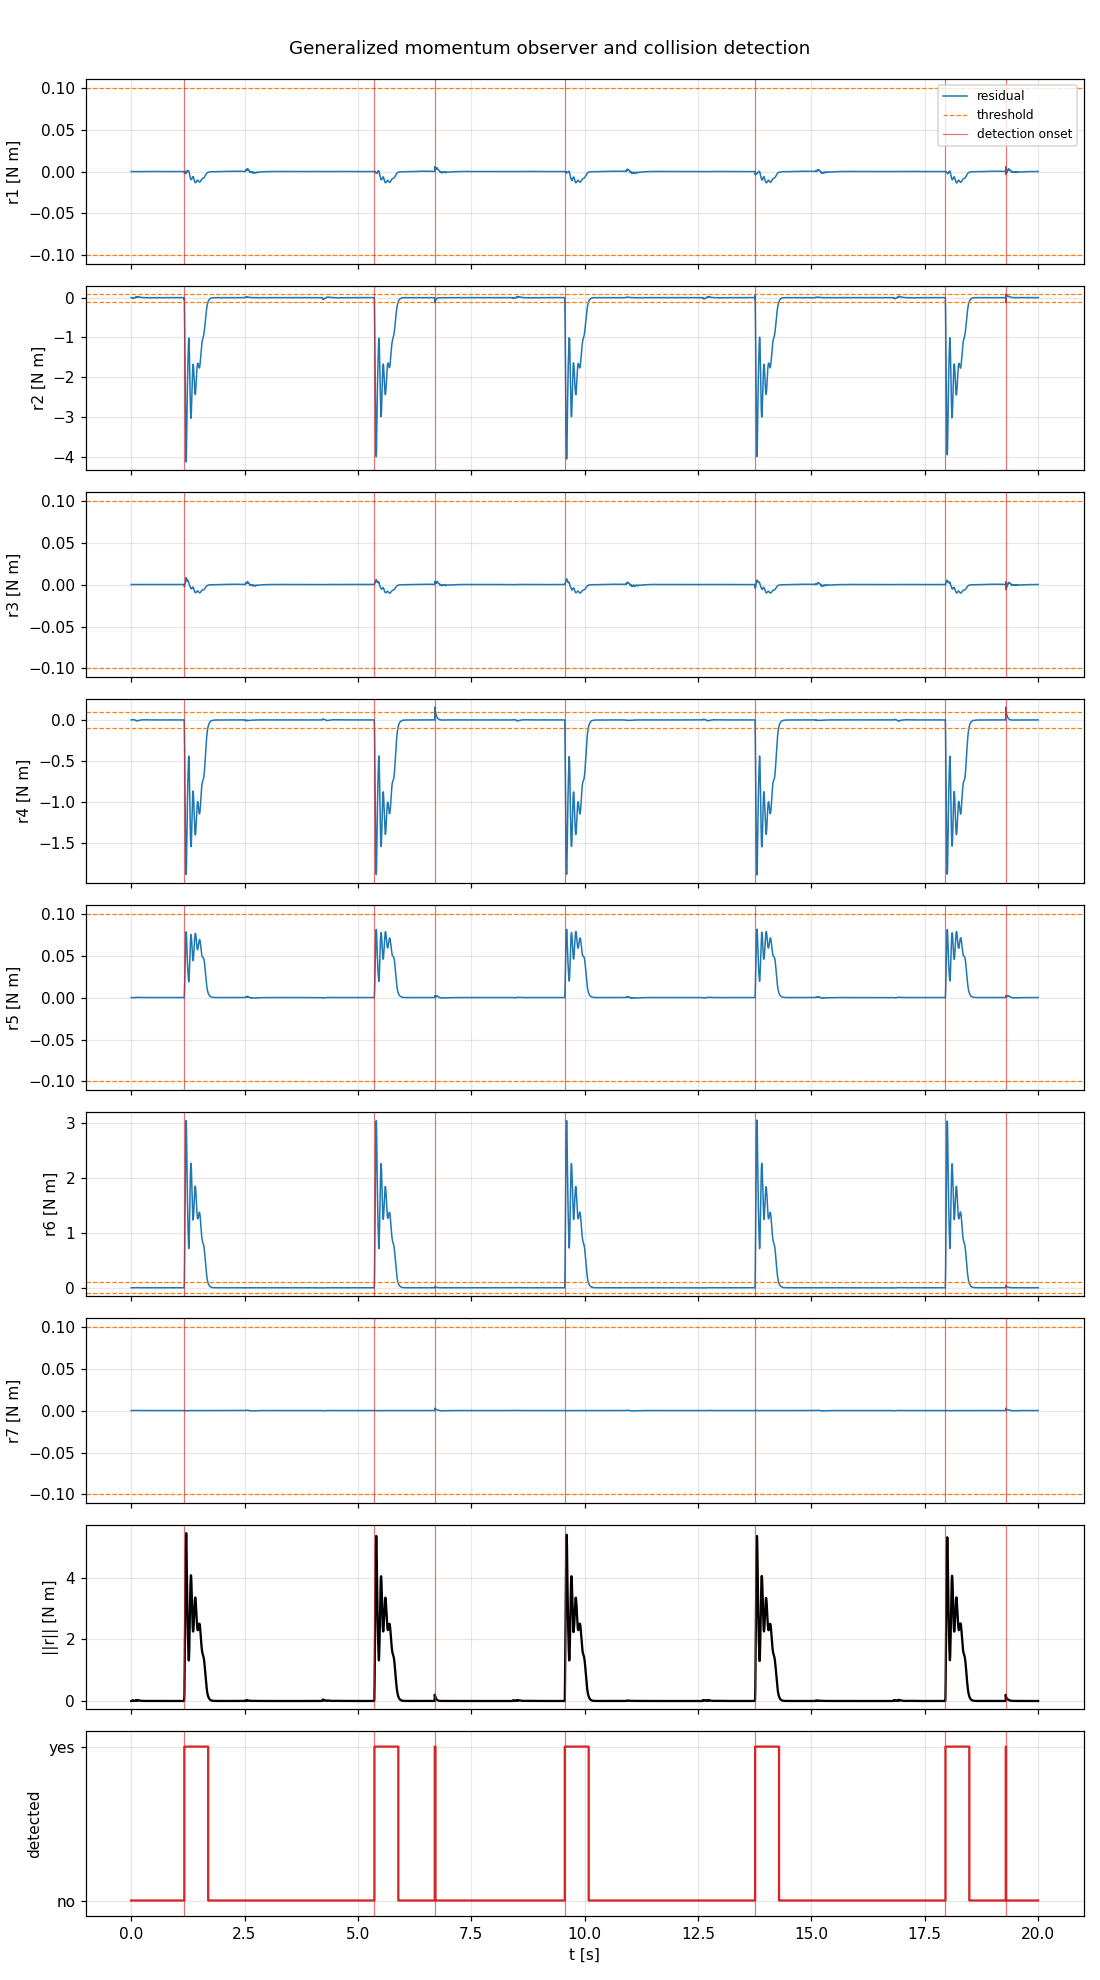
\includegraphics[height=0.82\textheight,keepaspectratio]{fig01_observer_before_return_ramp}
  \caption{Before the return ramp: the original circular full-online observer plot.
  Noncontact detection onsets occur at 6.694 and 19.286\,s.}
  \label{fig:obs-before}
\end{figure}

\begin{figure}[p]
  \centering
  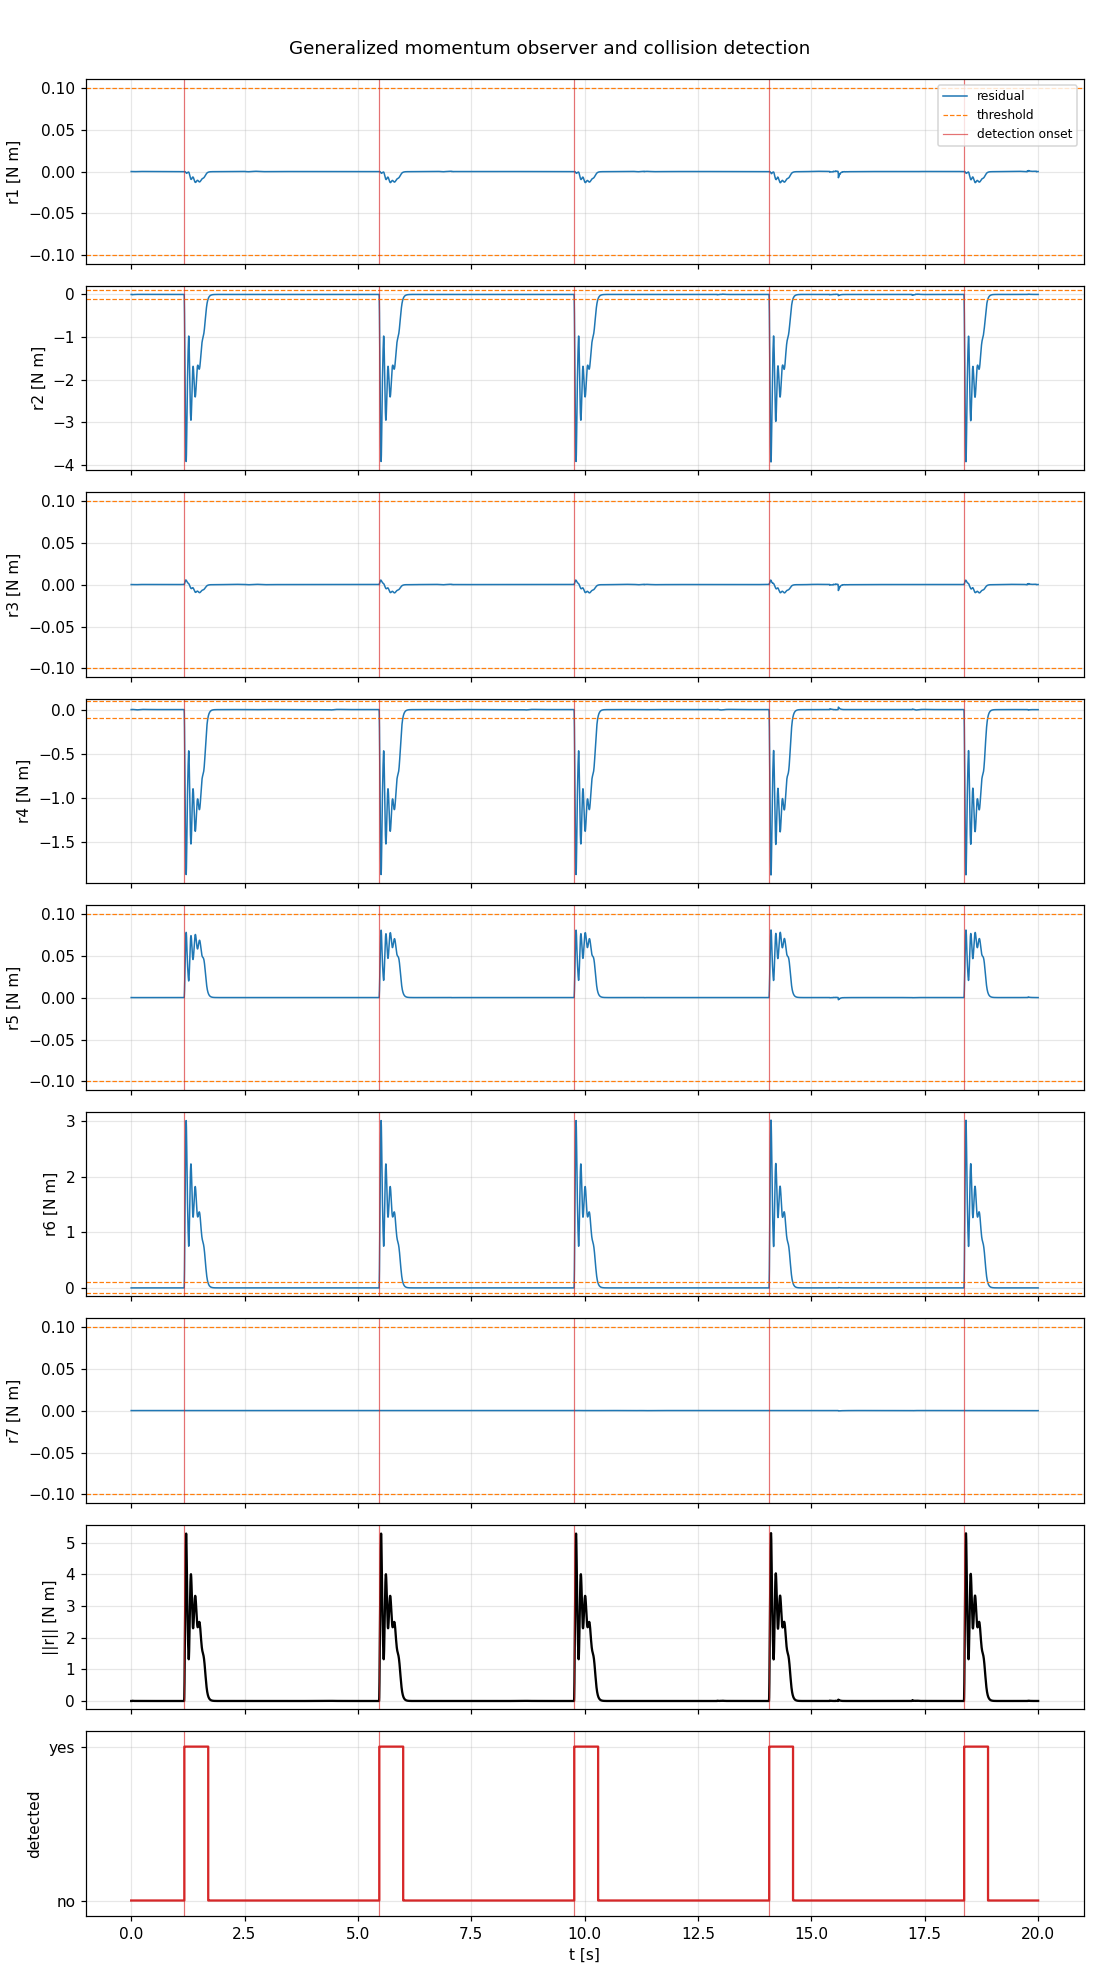
\includegraphics[height=0.82\textheight,keepaspectratio]{fig02_observer_after_return_ramp}
  \caption{Circular full-online observer response with the 0.20\,s return transition.}
  \label{fig:obs-after}
\end{figure}

\clearpage
\subsection{Contact force estimation}
Under nominal dynamics, the residual follows
$\dot r = K_O(\tau_{\mathrm{ext}}-r)$~\cite{haddadin2017}.
The gain of 30\,s$^{-1}$ gives a time constant of about 33\,ms. This
attenuates fast disturbances in the detection signal and also suppresses
short force peaks.

For offline force estimation, we invert the observer's implicit Euler update
at the logged sample interval $\Delta t_k = t_k - t_{k-1}$. For a single
contact at the fingertip along the known wall normal $n$, we project the
reconstructed joint torque onto $h_k=J_{\mathrm{tip}}(q_k)^{\mathsf T}n$.
\begin{equation}
  \widetilde{\tau}_{\mathrm{ext},k} =
    r_k + K_O^{-1}\frac{r_k-r_{k-1}}{\Delta t_k},
  \qquad
  \widehat F_{n,k} =
    \frac{h_k^{\mathsf T}\widetilde{\tau}_{\mathrm{ext},k}}{h_k^{\mathsf T}h_k}.
\end{equation}
The simulated force is the validation reference. The detector applies its
threshold to the filtered residual.

Figure~\ref{fig:force-estimation} uses the same full-online runs as the
impact comparison. Direct projection of the filtered residual underestimates
the first-impact peaks by 42--43\% and delays them by 20--21\,ms. Inversion
brings both peaks within 0.05\,N of the simulated peaks, with a remaining
delay of 2\,ms. The simulated force reaches its peak 24--27\,ms after contact,
before one observer time constant has elapsed. Inverting the low-pass dynamics
largely compensates for this attenuation under nominal conditions. The numerical
derivative of the residual amplifies measurement noise, and the reconstruction
also depends on the dynamic model and torque timing.

\begin{figure}[htbp]
  \centering
  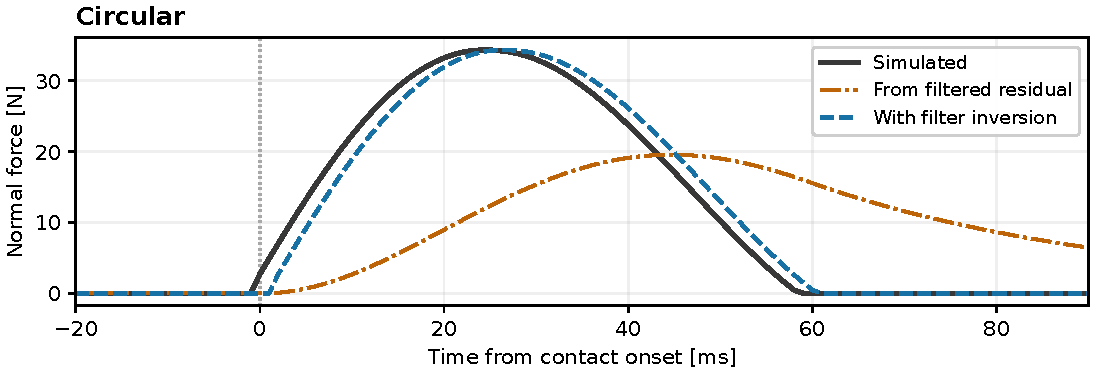
\includegraphics[width=0.94\linewidth]{fig09_force_estimation_circular}\par
  \medskip
  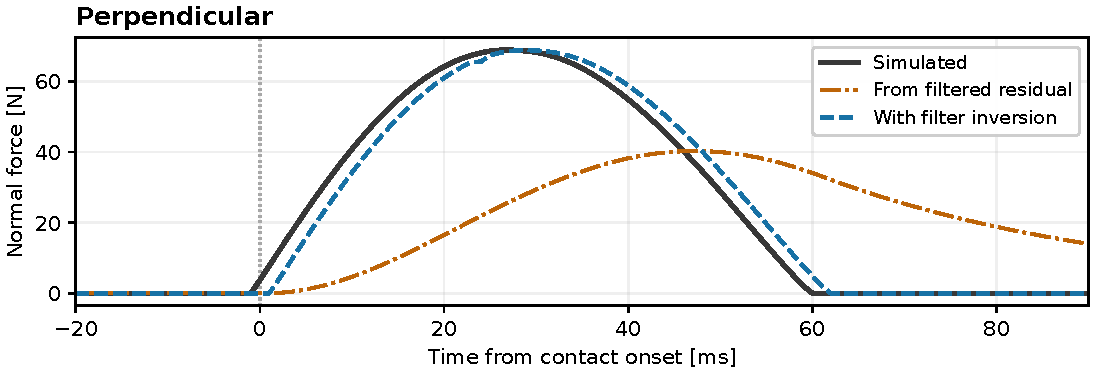
\includegraphics[width=0.94\linewidth]{fig10_force_estimation_perpendicular}
  \caption{Simulated and estimated normal force at first contact in the
  circular (top) and perpendicular (bottom) full-online runs.}
  \label{fig:force-estimation}
\end{figure}

% =====================================================================
\clearpage
\section{Elastic Model of the First Impact}
\label{sec:elastic}

The elastic model describes a one-dimensional impact. A constant mass $\ms$, equal
to the directional effective mass at the last sample before contact, strikes an undamped
linear spring of stiffness $k_e = 20\,000$\,N/m at normal speed $\vs$. The penetration
$\delta$ starts at $\delta(0)=0$ with $\dot\delta(0)=\vs$ and satisfies
\begin{equation}
  \ms \ddot\delta + k_e \delta = 0, \qquad F_n = k_e\,\delta .
  \label{eq:elastic-model}
\end{equation}
The solution is $\delta(t) = (\vs/\omega)\sin\omega t$ with $\omega=\sqrt{k_e/\ms}$.
Contact ends after half an oscillation, when the spring returns to zero compression.
The resulting contact duration, peak force and impulse are
\begin{align}
  T_{\mathrm{el}} &= \frac{\pi}{\omega} = \pi\sqrt{\frac{\ms}{k_e}},
  \label{eq:elastic-T}\\
  F_{\mathrm{peak,el}} &= k_e\,\frac{\vs}{\omega} = \vs\sqrt{k_e\, \ms},
  \label{eq:elastic-F}\\
  I_{\mathrm{el}} &= \int_0^{T_{\mathrm{el}}} F_n(t)\,dt
     = \ms \vs \int_0^{\pi} \sin s\, ds = 2\, \ms \vs .
  \label{eq:elastic-I}
\end{align}
The impulse in \eqref{eq:elastic-I} is the change in momentum when the mass rebounds
at the same speed in the opposite direction.

At fixed pre-impact normal velocity and wall stiffness, a fractional effective mass
reduction $\Delta_m$ gives $m_n^{-,\mathrm{opt}} = (1-\Delta_m)\, m_n^{-,\mathrm{base}}$.
Equations~\eqref{eq:elastic-T}--\eqref{eq:elastic-I} then give
\begin{equation}
  \frac{F^{\mathrm{opt}}_{\mathrm{peak}}}{F^{\mathrm{base}}_{\mathrm{peak}}}
  = \frac{T^{\mathrm{opt}}}{T^{\mathrm{base}}} = \sqrt{1-\Delta_m},
  \qquad
  \frac{I^{\mathrm{opt}}}{I^{\mathrm{base}}} = 1-\Delta_m .
  \label{eq:elastic-ratio}
\end{equation}
Peak force and contact duration scale with the square root of the pre-impact
effective mass, and impulse scales linearly. At $\Delta_m = 30\%$, the expected peak-force
reduction is $1-\sqrt{0.70} = 16.3\%$ and the expected impulse reduction is $30\%$.

Section~\ref{sec:elastic-compare} evaluates the predictions using the measured
effective mass and normal velocity of each run.

% =====================================================================
\section{Circular Experiment}

\subsection{First compression-release cycle}

\begin{table}[htbp]
  \centering
  \begin{tabular}{lrrr}
    \toprule
    Metric & Baseline & Full online & Change (\%) \\
    \midrule
    Contact onset (s)            & 1.167   & 1.167   & -- \\
    Effective mass at impact (kg)    & 7.189   & 4.623   & $-35.69$ \\
    Pre-impact normal velocity (m/s) & 0.10893 & 0.10893 & $-0.0027$ \\
    Pre-impact normal energy (mJ)    & 42.656  & 27.430  & $-35.69$ \\
    Peak force (N)               & 43.147  & 34.354  & $-20.38$ \\
    First-cycle impulse (N\,s)   & 2.1017  & 1.2581  & $-40.14$ \\
    Peak penetration (mm)        & 2.155   & 1.714   & $-20.44$ \\
    First-cycle duration (ms)    & 84.0    & 59.0    & $-29.76$ \\
    Precontact RMS error (mm)    & 0.0190  & 0.0231  & $+21.60$ \\
    \bottomrule
  \end{tabular}
  \caption{Circular experiment: first compression-release cycle.}
  \label{tab:circ}
\end{table}

In the circular test, the peak force drops by 20.38\% and the first
compression-release cycle shortens from 84 to 59\,ms. The mean force over
this cycle drops from 25.0 to 21.3\,N. Together, the lower mean force and
earlier release reduce the first-cycle impulse by about 40\%.

\begin{figure}[p]
  \centering
  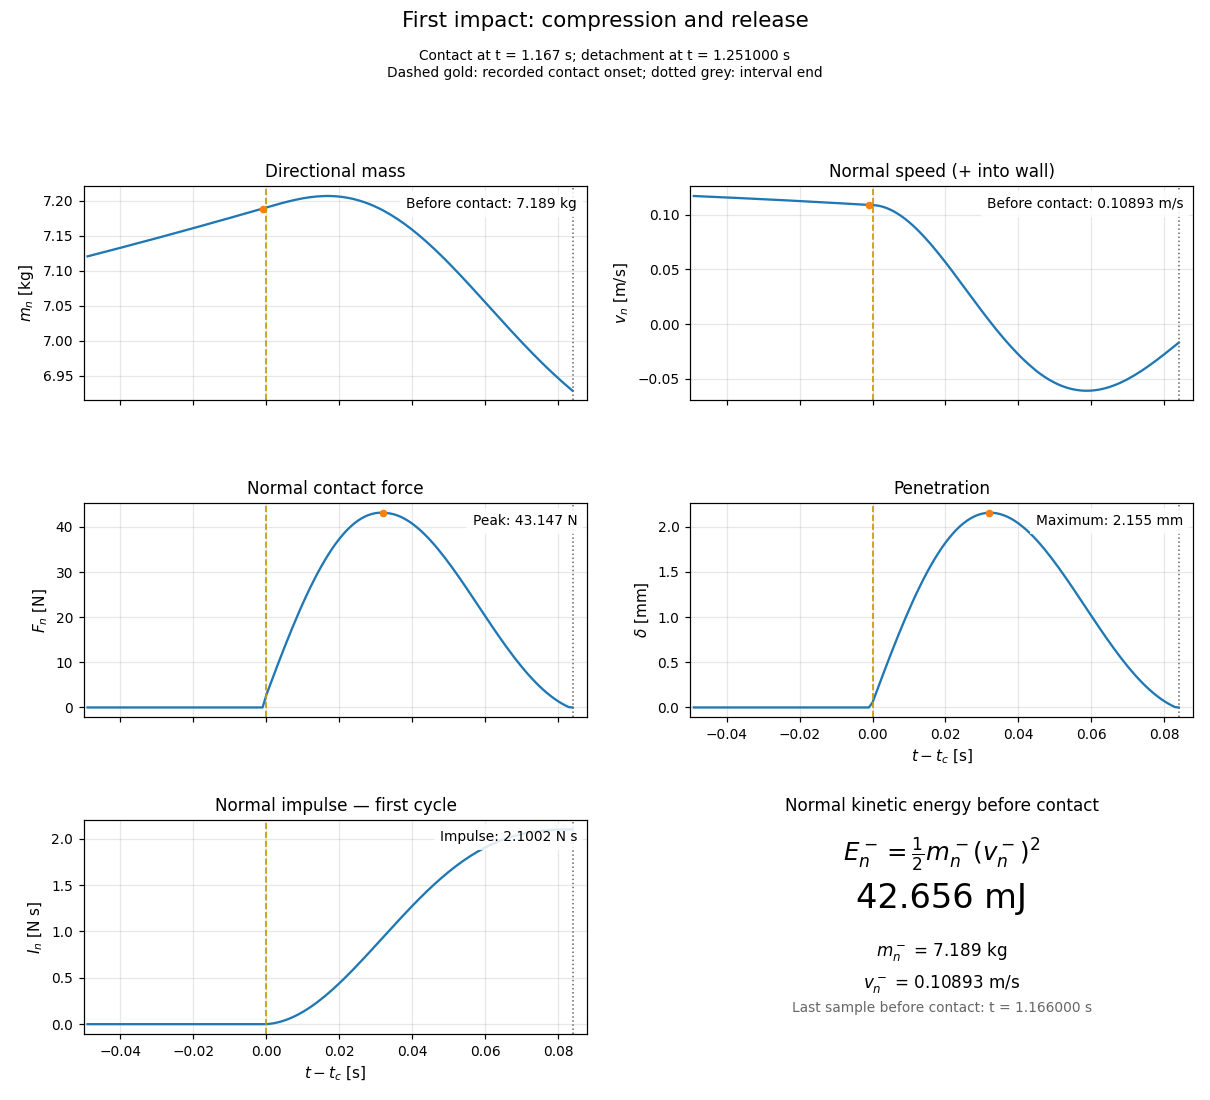
\includegraphics[width=\textwidth]{fig03_circular_baseline_first_impact}
  \caption{Circular baseline: first impact in the run with the shared RETURN schedule.}
  \label{fig:circ-base-first}
\end{figure}

\begin{figure}[p]
  \centering
  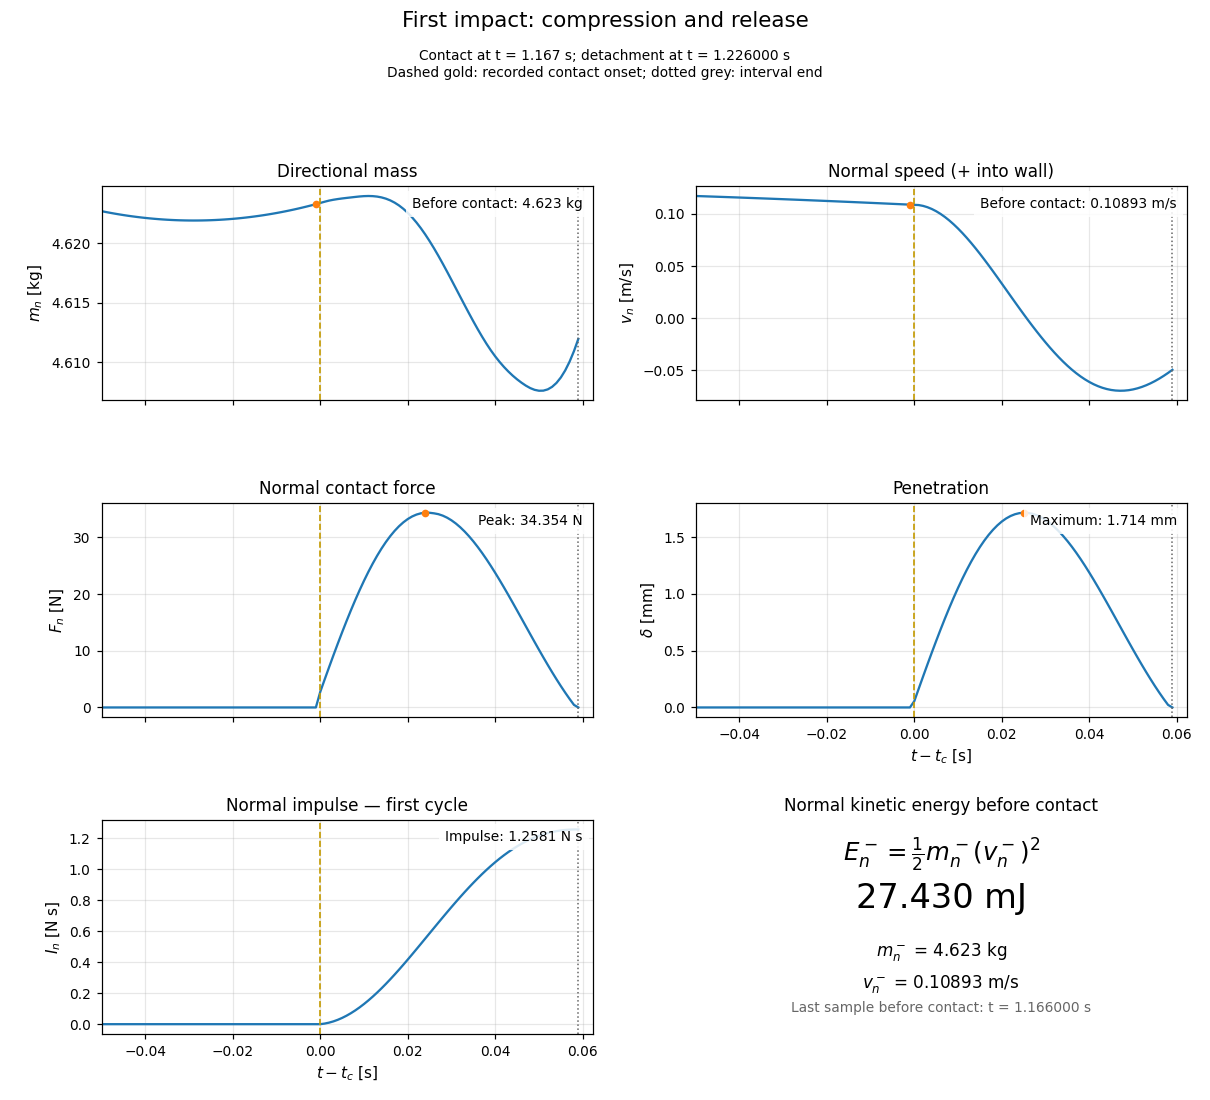
\includegraphics[width=\textwidth]{fig04_circular_online_first_impact}
  \caption{Circular full-online controller: first impact in the run with the shared
  RETURN schedule.}
  \label{fig:circ-opt-first}
\end{figure}

\subsection{Repeated circles and return scheduling}
Figures~\ref{fig:circ-base-all} and~\ref{fig:circ-opt-all} show all contacts in the
same 20\,s runs used for the first-impact comparison. With the shared RETURN schedule,
the first contacts match on all five approaches, starting at 1.167\,s and recurring
every 4.5\,s. The full-online recontacts occur 2\,ms earlier than the corresponding
baseline recontacts. No contacts occur during RETURN.

\begin{figure}[p]
  \centering
  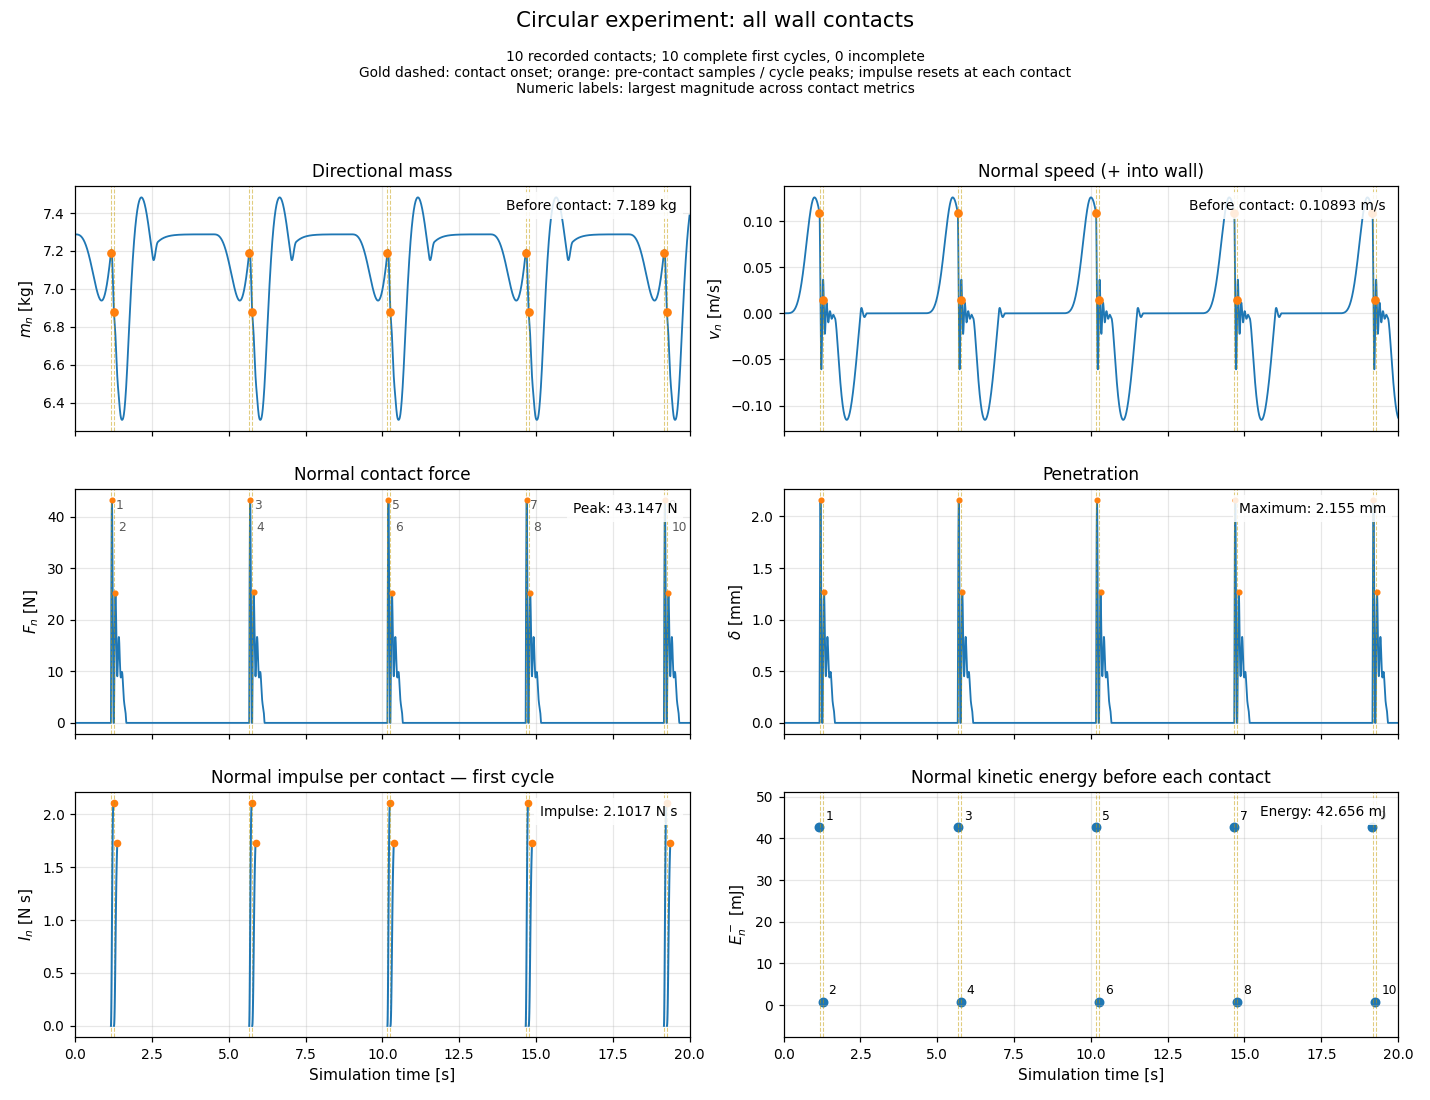
\includegraphics[width=\textwidth]{fig05_circular_baseline_all_collisions}
  \caption{Circular baseline: all contacts over 20\,s with the shared RETURN schedule.}
  \label{fig:circ-base-all}
\end{figure}

\begin{figure}[p]
  \centering
  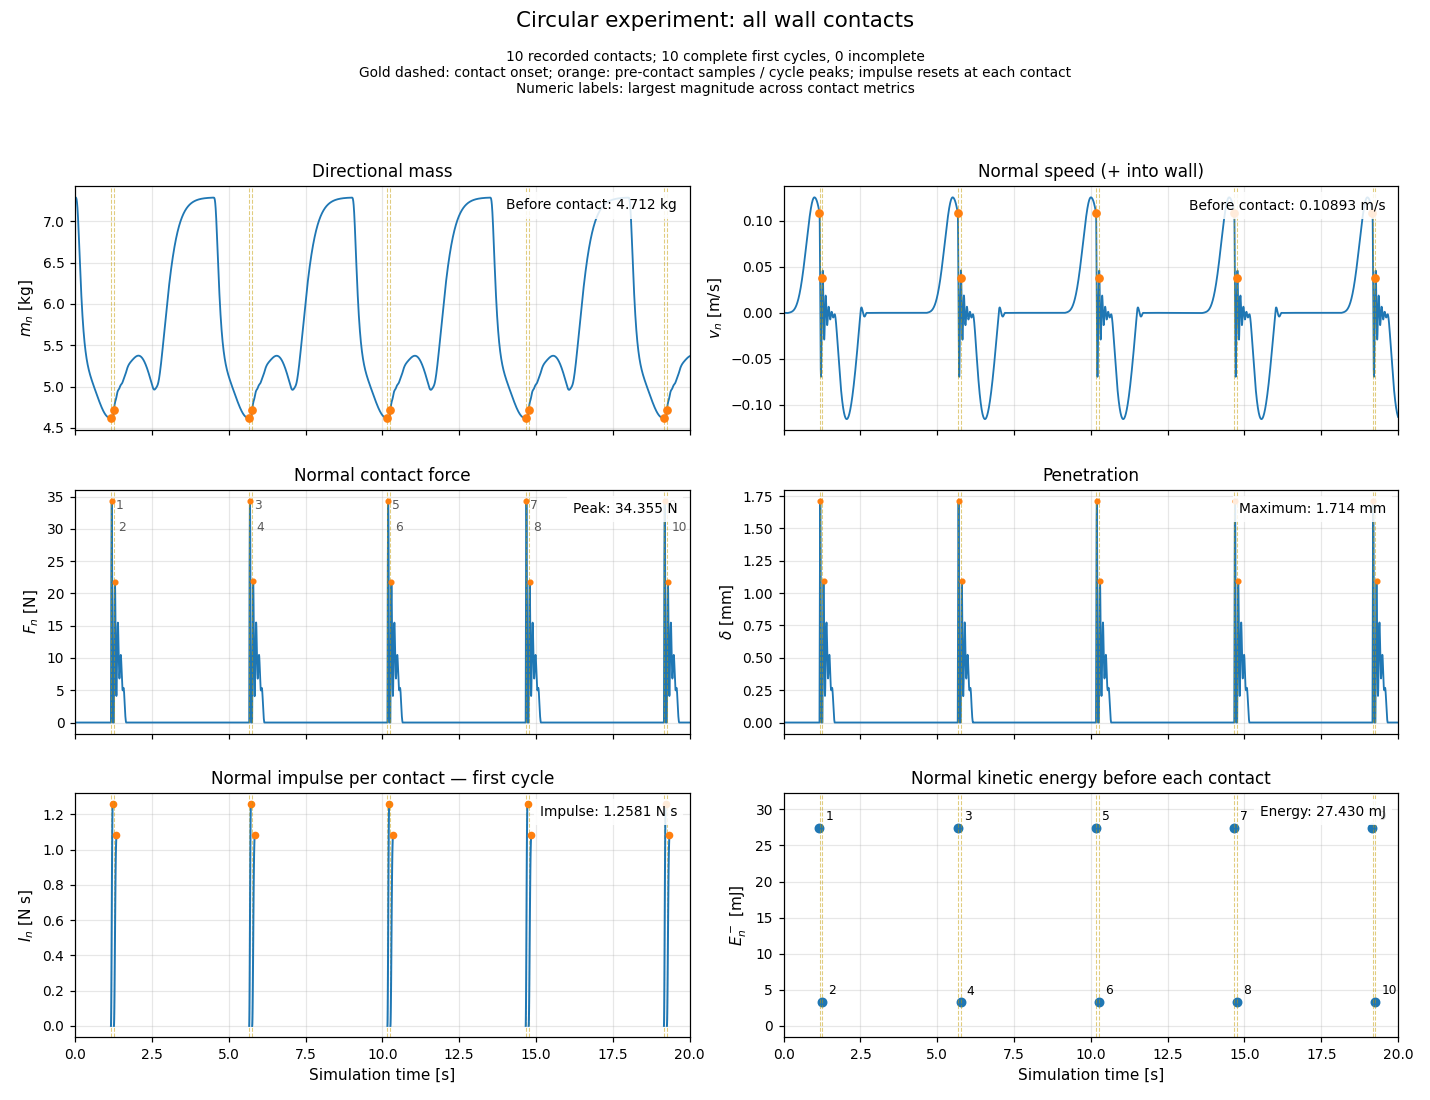
\includegraphics[width=\textwidth]{fig06_circular_online_all_collisions}
  \caption{Circular full-online controller: all contacts over 20\,s with the shared
  RETURN schedule.}
  \label{fig:circ-opt-all}
\end{figure}

% =====================================================================
\clearpage
\section{Perpendicular Experiment}

\begin{table}[htbp]
  \centering
  \begin{tabular}{lrrr}
    \toprule
    Metric & Baseline & Full online & Change (\%) \\
    \midrule
    Contact onset (s)            & 0.350   & 0.350   & -- \\
    Effective mass at impact (kg)    & 7.622   & 5.182   & $-32.02$ \\
    Pre-impact normal velocity (m/s) & 0.20003 & 0.19996 & $-0.0332$ \\
    Pre-impact normal energy (mJ)    & 152.484 & 103.596 & $-32.06$ \\
    Peak force (N)               & 85.235  & 68.909  & $-19.15$ \\
    First-cycle impulse (N\,s)   & 3.5438  & 2.6406  & $-25.49$ \\
    Peak penetration (mm)        & 4.256   & 3.438   & $-19.20$ \\
    First-cycle duration (ms)    & 64.0    & 60.0    & $-6.25$ \\
    Precontact RMS error (mm)    & 0.1011  & 0.0861  & $-14.81$ \\
    \bottomrule
  \end{tabular}
  \caption{Perpendicular experiment: first compression-release cycle.}
  \label{tab:perp}
\end{table}

The perpendicular contact duration changes by only 4\,ms, from 64 to 60\,ms.
Most of the 25.49\% reduction in impulse comes from the lower mean normal
force over that interval, which falls from 55.4 to 44.0\,N.

The pre-impact Cartesian position RMS error stays below 0.11\,mm in all four runs.
With the full-online controller, it rises by 4.1\,$\mu$m in the circular experiment
and falls by 15.0\,$\mu$m in the perpendicular experiment. The effective mass
reduction is therefore achieved with comparable primary tracking accuracy in
these nominal runs.

\begin{figure}[p]
  \centering
  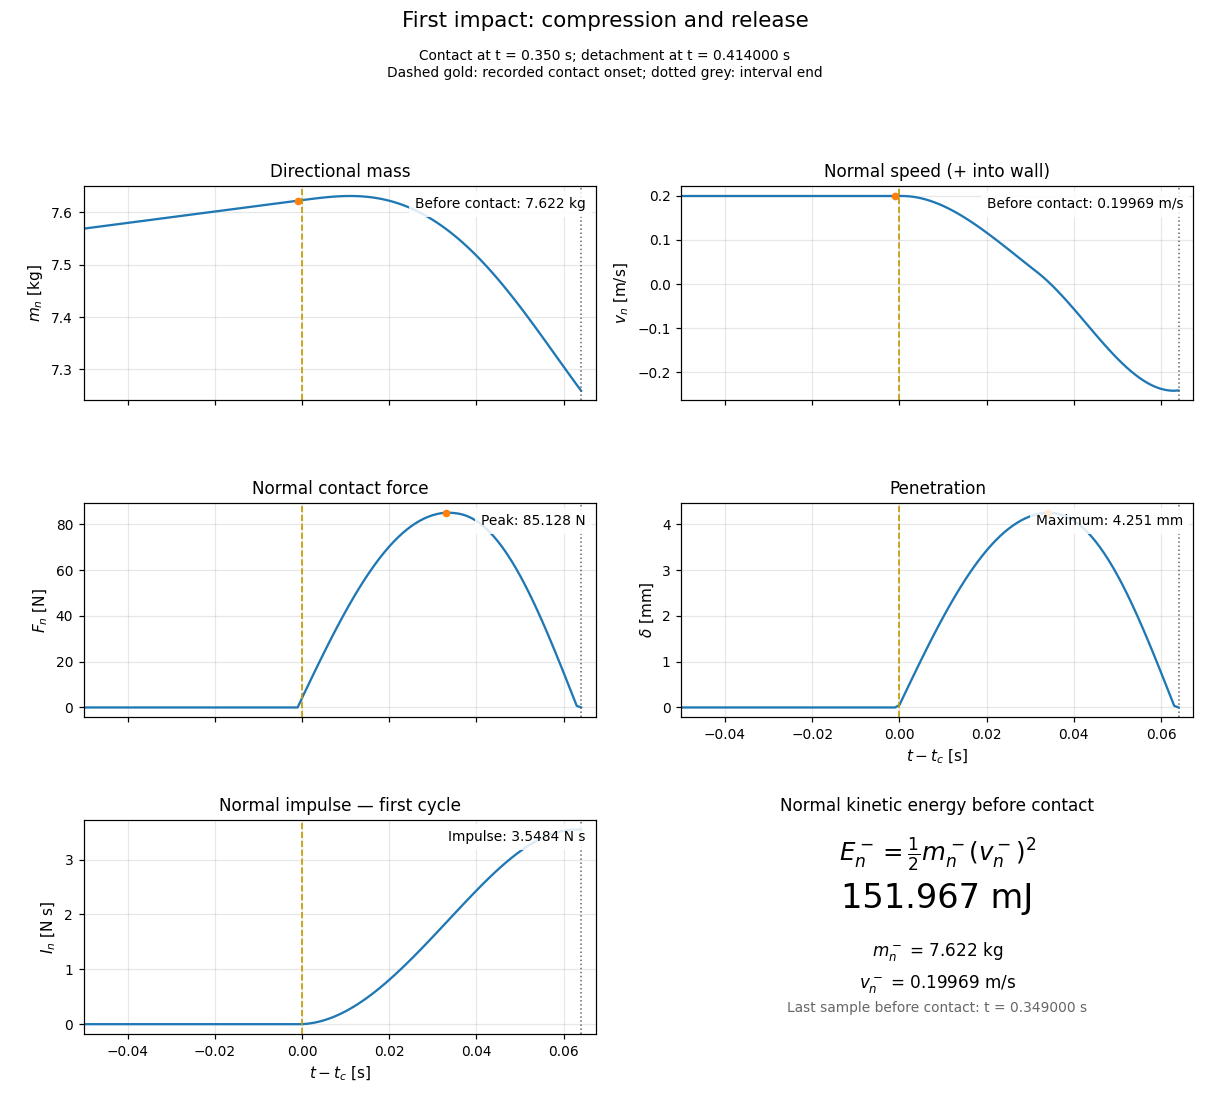
\includegraphics[width=\textwidth]{fig07_perpendicular_baseline_first_impact}
  \caption{First impact with the perpendicular baseline controller.}
  \label{fig:perp-base}
\end{figure}

\begin{figure}[p]
  \centering
  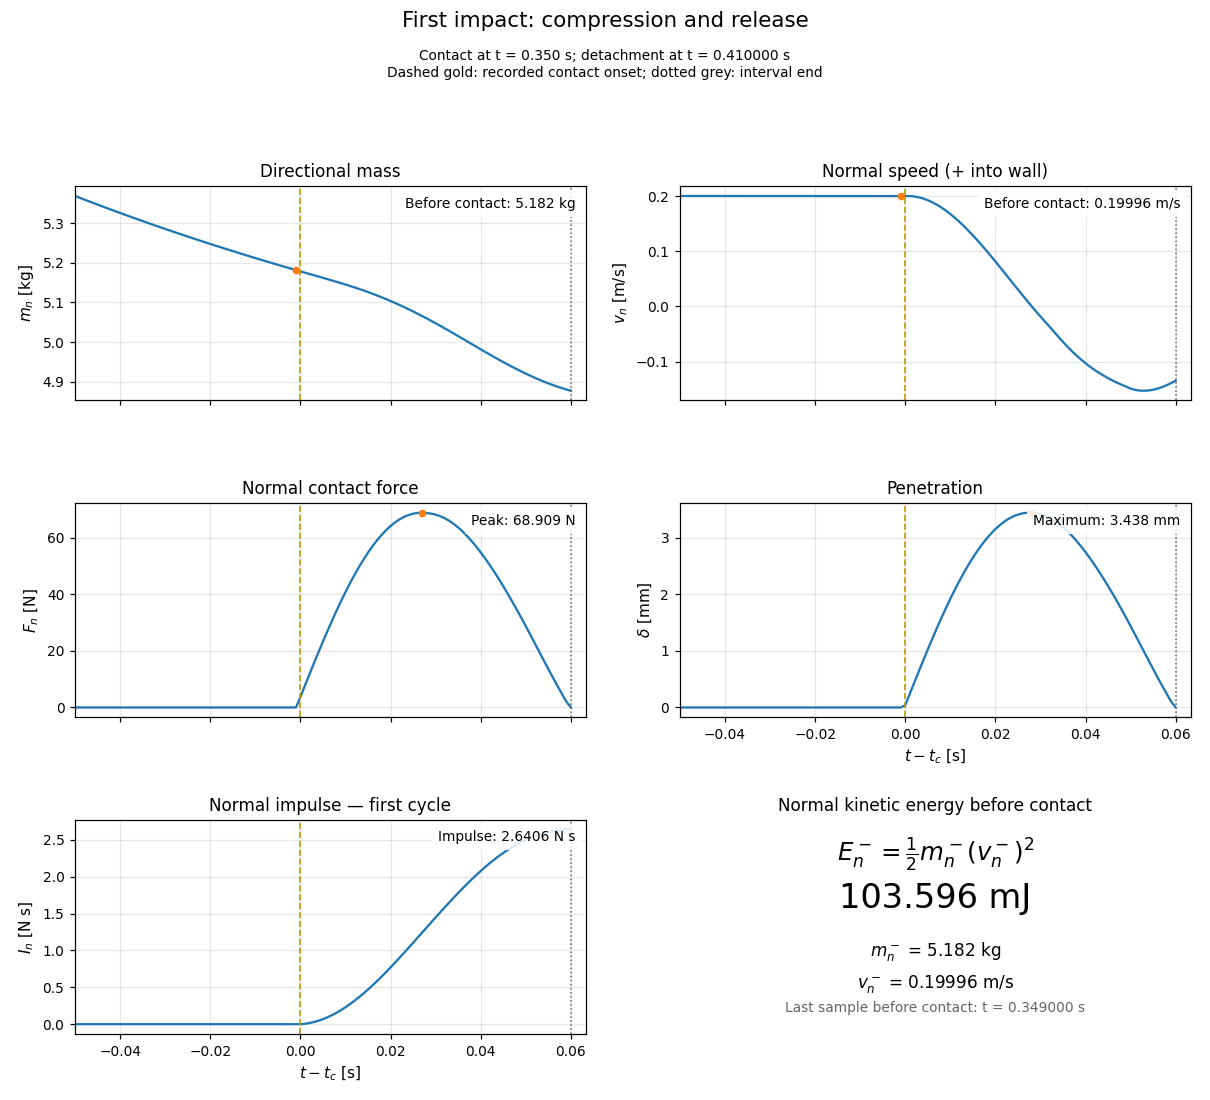
\includegraphics[width=\textwidth]{fig08_perpendicular_online_first_impact}
  \caption{First impact with the perpendicular full-online controller.}
  \label{fig:perp-opt}
\end{figure}

% =====================================================================
\clearpage
\section{Measured vs.\ Predicted Impact Reductions}
\label{sec:elastic-compare}

The elastic predictions use the measured pre-impact effective mass and normal velocity
of each run, with $k_e = 20\,000$\,N/m. Table~\ref{tab:elastic-compare} compares the
predicted force, impulse and contact duration with the simulated values.

\begin{table}[htbp]
  \centering
  \small
  \setlength{\tabcolsep}{5pt}
  \begin{tabular}{lrrrrrr}
    \toprule
     & \multicolumn{3}{c}{Elastic prediction}
     & \multicolumn{3}{c}{Simulation measurement} \\
    \cmidrule(lr){2-4}\cmidrule(lr){5-7}
    Quantity & Baseline & Full online & Change (\%)
             & Baseline & Full online & Change (\%) \\
    \midrule
    \multicolumn{7}{l}{\emph{Circular} ($\Delta_m = 35.69\%$)} \\
    Peak force (N)     & 41.31 & 33.12 & $-19.81$ & 43.15 & 34.35 & $-20.38$ \\
    Impulse (N\,s)     & 1.566 & 1.007 & $-35.69$ & 2.102 & 1.258 & $-40.14$ \\
    Duration (ms)      & 59.6  & 47.8  & $-19.81$ & 84.0  & 59.0  & $-29.76$ \\
    \midrule
    \multicolumn{7}{l}{\emph{Perpendicular} ($\Delta_m = 32.02\%$)} \\
    Peak force (N)     & 78.10 & 64.37 & $-17.58$ & 85.24 & 68.91 & $-19.15$ \\
    Impulse (N\,s)     & 3.049 & 2.072 & $-32.04$ & 3.544 & 2.641 & $-25.49$ \\
    Duration (ms)      & 61.3  & 50.6  & $-17.55$ & 64.0  & 60.0  & $-6.25$ \\
    \bottomrule
  \end{tabular}
  \caption{First impact: elastic prediction \eqref{eq:elastic-T}--\eqref{eq:elastic-I}
  against the simulated first compression-release cycle.}
  \label{tab:elastic-compare}
\end{table}

\paragraph{Peak force.}
The elastic model estimates the peak-force reduction within 1.6 percentage points
in both comparisons.

\paragraph{Impulse and contact duration.}
The simulation gives a larger reduction in contact duration for the circular
experiment (29.76\% versus 19.81\% predicted) and a smaller reduction for the
perpendicular experiment (6.25\% versus 17.55\%). This partly explains the
differences between the predicted and simulated impulse reductions.

The measured impulses are 16--34\% larger than $2\,\ms \vs$. The elastic model
assumes a constant mass coupled to an undamped spring with no actuation.
In the simulation, the wall damping ratio
$\zeta = c_e/(2\sqrt{k_e \ms}) \approx 0.02$ is small, the controller continues
applying torques to track the reference during contact, and $m_n(q)$ changes
as the robot moves. Continued actuation can push the fingertip toward the wall
during contact, which may prolong contact and increase the resulting impulse.

% =====================================================================
\section{Constraints, Fallbacks and Execution Timing}

\begin{table}[htbp]
  \centering
  \begin{tabular}{lccccc}
    \toprule
    Optimized run & \multicolumn{3}{c}{QP failures} & Min margin & Clipped \\
    \cmidrule(lr){2-4}
                  & Safety & Tracking & Secondary & (rad) & samples \\
    \midrule
    Circular      & 0 & 0 & 0  & 0.148855 & 0 \\
    Perpendicular & 0 & 0 & 38 & 0.151151 & 0 \\
    \bottomrule
  \end{tabular}
  \caption{QP failures, margins and clipping for the optimized runs.}
  \label{tab:qp}
\end{table}

The 38 perpendicular secondary fallbacks occur between 0.382 and 0.419\,s,
after contact begins at 0.350\,s. All 38 solves reach the 1000-iteration limit.
The log records 34 inaccurate primal-infeasibility statuses
and four entries with status $-2$, which can indicate either the iteration
limit or rejection by the controller's numerical checks. Level 3 must
satisfy $Ju=Ju_2$ together with the inherited bounds. The level-2 solution
satisfies that equality by construction, and its bounds are checked to
numerical tolerances. The log lacks the rejected iterates and their equality
errors, so it cannot distinguish the causes of the four $-2$ entries or
establish exact infeasibility.

At each fallback, the controller uses that update's verified level-2 solution.
This preserves the achieved tracking acceleration and skips secondary
optimization for that update. The pre-impact effective mass is measured before
the first fallback. The recorded contact force includes their effects.

The maximum normalized slack exceeds $10^{-6}$ on about 1.84\% of
circular optimized updates and 17.73\% of perpendicular optimized
updates. Acceleration estimates from finite differences of the logged
velocities reach about 29.93\,rad/s$^2$ in the circular optimized run and
49.55\,rad/s$^2$ in the perpendicular optimized run. The corresponding
baseline maxima are 23.80 and 43.91\,rad/s$^2$. The perpendicular optimized
run exceeds the soft acceleration preference of 30\,rad/s$^2$ during contact.

The minimum physical margin in the circular optimized run is 0.14885\,rad.
It briefly falls below the preferred 0.15\,rad margin and stays above the
0.06\,rad hard margin. The perpendicular optimized run has a minimum margin
of 0.15115\,rad. Every recorded sample in both optimized runs satisfies the
hard position and velocity limits, with no actuator clipping.

\begin{table}[htbp]
  \centering
  \begin{tabular}{lcccc}
    \toprule
    Run & \begin{tabular}[c]{@{}c@{}}Update mean\\(ms)\end{tabular}
        & \begin{tabular}[c]{@{}c@{}}p95\\(ms)\end{tabular}
        & \begin{tabular}[c]{@{}c@{}}Update max\\(ms)\end{tabular}
        & \begin{tabular}[c]{@{}c@{}}Missed samples\\(\%)\end{tabular} \\
    \midrule
    Circular baseline      & 0.352 & 0.516 &  4.783 & 5 (0.025) \\
    Circular online        & 0.815 & 1.107 & 29.892 & 7 (0.035) \\
    Perpendicular baseline & 0.416 & 0.618 & 9.761  & 1 (0.177) \\
    Perpendicular online   & 0.994 & 1.610 & 2.709  & 0 (0.000) \\
    \bottomrule
  \end{tabular}
  \caption{Controller update timing.}
  \label{tab:timing}
\end{table}

At RTF 0.20, a 1\,ms simulated step corresponds to about 5\,ms of wall time.
The 95th-percentile update times of the circular and perpendicular full-online
controllers are 1.107 and 1.610\,ms, respectively. Each already exceeds the
entire 1\,ms period of a physical 1\,kHz loop.

The virtual wall applies force only at the fingertip. The geometric penetration
estimate uses bounding boxes around the hand and fingers. It first becomes positive
about 32\,ms before fingertip contact in the circular full-online run and 13\,ms
before it in the perpendicular run. The maximum estimated overlaps over the
complete runs are 5.34 and 9.25\,mm, respectively.

% =====================================================================
\clearpage
\section{Conclusions}
The full-online HQP controller exploits the redundancy of the FR3 while
tracking the fingertip position. At comparable pre-impact normal velocities,
the effective mass falls by 35.69\% in the circular experiment and 32.02\% in
the perpendicular experiment, meeting the 30\% target in both cases. Peak
force drops by 20.38\% and 19.15\%, respectively, and the first-cycle impulse
falls by 40.14\% and 25.49\%.

The peak-force reductions agree with the scaling predicted by the
one-dimensional elastic model. Impulse and contact duration depart more
from the predictions because the force history also depends on the control
action during contact and the variation of effective mass with posture.

A major limitation of the simulation is the assumption of fingertip-only contact.
The position task leaves the hand orientation free, and the estimated
geometric overlap starts before fingertip contact in both full-online runs.
If the hand reaches the wall first, the impact configuration and contact
Jacobian change, along with the effective mass at the point of
contact~\cite{haddadin2017}. A model that includes hand and link contact
would support evaluation of orientation or clearance constraints. Those
constraints would restrict the feasible configurations available for effective
mass optimization.

The 95th-percentile update times of both full-online controllers exceed
the 1\,ms period of the Franka Control Interface at 1\,kHz~\cite{franka-fci}.
Feasibility on the target hardware therefore requires timing the complete
torque loop, including observer and communication costs, and measuring
latency and missed deadlines during contact.

All simulations were performed under nominal dynamics. The sensitivity of
the controller to joint friction, inertial parameter uncertainties and
measurement noise remains to be investigated. This matters for the momentum
observer because errors in the estimated external torque also affect the
constraint prediction within the HQP.

% =====================================================================

\clearpage
\begin{thebibliography}{9}
\phantomsection
\addcontentsline{toc}{section}{References}
\bibitem{khatib1987}
O.~Khatib, ``A unified approach for motion and force control of robot manipulators:
The operational space formulation,'' \emph{IEEE Journal on Robotics and Automation},
vol.~3, no.~1, pp.~43--53, 1987.

\bibitem{haddadin2017}
S.~Haddadin, A.~De~Luca, and A.~Albu-Sch\"affer, ``Robot collisions: A survey on
detection, isolation, and identification,'' \emph{IEEE Transactions on Robotics},
vol.~33, no.~6, pp.~1292--1312, 2017.

\bibitem{deluca2005}
A.~De~Luca and R.~Mattone, ``Sensorless robot collision detection and hybrid
force/motion control,'' in \emph{Proc. IEEE Int. Conf. on Robotics and Automation
(ICRA)}, 2005, pp.~999--1004.

\bibitem{franka-fci}
Franka Robotics, ``libfranka Overview,'' \emph{Franka Control Interface documentation}.
\url{https://frankarobotics.github.io/docs/doc/libfranka/docs/overview.html}.
\end{thebibliography}

\end{document}
